%=================================================================================================%
% This is a template designed for Chin. Phys. B (Dated 12 November 2014)
% Only one step to compile: PDFTeXify
%=================================================================================================%
\documentclass{cpbtex3}
\usepackage{graphicx}% Include figure files
\usepackage{dcolumn}% Align table columns on decimal point
\usepackage{bm}% bold math
\usepackage{authblk}
%\usepackage[backend=biber]{biblatex}
%\usepackage[mathlines]{lineno}% Enable numbering of text and display math
%\linenumbers\relax % Commence numbering lines
\usepackage{titlesec}      % For customizing section titles
% ===== 1. Small font for affiliations =====
\renewcommand{\Affilfont}{\small} % Set affiliation font size to small

% ===== 2. Bold abstract title =====
\usepackage{abstract} % Required to modify abstract title formatting
\renewcommand{\abstitlestyle}[1]{{\centering\bfseries #1\par}} % Bold + centered

% ===== 3. Automatically bold ALL titles (section/subsection/abstract) =====
\titleformat*{\section}{\bfseries}     % Bold sections
\titleformat*{\subsection}{\bfseries}  % Bold subsections
\titleformat*{\subsubsection}{\bfseries} % Bold subsubsections


\graphicspath{{Figure/}}
\usepackage{fontspec}
\setCJKmainfont{SimSun}[AutoFakeBold=true]  % Use SimSun or other available Chinese font
%\setmainfont{Times New Roman}  % Main English font

%\usepackage[utf8]{inputenc}
%\usepackage[T1]{fontenc}
\usepackage{mathptmx}
\usepackage{etoolbox}
\usepackage{microtype} 
\usepackage{caption}
\usepackage{hyperref}
\captionsetup[figure]{labelfont=bf, name=Fig., labelsep=period}
\bibliographystyle{iopart-num} 
\graphicspath{{Figure/}}

\begin{document}


\title{Analysis of the Anomalous Doppler Effect from Quantum Theory to Classical Dynamics Simulations}

% Title should be concise; avoid abbreviations if possible; and not begin with `A', `An', `The', or `Study on'.

%\author{Xinhang Xu (徐新航)$^{1}$, \ Jian Liu (刘健)$^{2}$,  \ Wandong Liu (刘万东)$^{1}$, \ and   \ Jinlin Xie (谢锦林)$^{1},$ \thanks{Corresponding author. E-mail:jlxie@ustc.edu.cn}\\
%%\author{Xinhang Xu (徐新航)$^{1}$, Second Author$^{2}$, $\ldots$, and Last Author$^{2,3,}$\thanks{Corresponding author. E-mail: xxx@xxx.edu}\\
%$^{1}${Department of plasma physics and fusion engineering, University of Science and Technology of China    
% Hefei  230026 , China}\\  % The line break was forced via \\
%$^{2}${Weihai Institute for Interdisciplinary Research, Shandong University, Weihai 264209, China} % The line break was forced via \\

\author{
Xinhang Xu (徐新航)$^{1}$, 
Jinlin Xie (谢锦林)$^{1}$\thanks{Corresponding author. E-mail: jlxie@ustc.edu.cn},
Jian Liu (刘健)$^{2}$, 
and Wandong Liu (刘万东)$^{1}$\\
$^{1}$Department of Plasma Physics and Fusion Engineering, University of Science and Technology of China, Hefei 230026, China \\
$^{2}$Weihai Institute for Interdisciplinary Research, Shandong University, Weihai 264209, China
}
% 1. For Chinese authors, the name in Chinese characters should also be given. For example, Gang Liu(����), Xiao-Ming Li(������)
% 2. Please ensure that every author approves the submission of the manuscript
% 3. Abbreviations should not be used in the affiliations

\date{\today}
\maketitle

\begin{abstract}
A quantum model incorporating angular momentum conservation is developed to analyze the Normal and Anomalous Doppler Effects, demonstrating that the resonance condition is strongly influenced by the angular momentum of the wave. The resonance condition involving wave angular momentum is examined numerically, and the energy exchange ratio between the electron's parallel and gyrokinetic motion during resonance with the electromagnetic wave is simulated, exhibiting strong agreement with quantum theoretical predictions.
\end{abstract}

\textbf{Keywords: Anomalous Doppler Effect, Resonant condition, Angular monmentum Conservation } %no more than four sets of keywords should be provided

\textbf{PACS:} %no more than four PACS codes should be provided: check https://cpb.iphy.ac.cn/UserFiles/File/PACS2010Regular-Edition.pdf


\section{Introduction}
The Anomalous Doppler Effect (ADE) \cite{tamm1959general,frank1960optics,ginzburg1960certain,shustin1971transformation}, in which the observed frequency shift behaves contrary to the conventional Doppler Effect under specific conditions, was first theoretically predicted by Soviet physicist Vitaly L. Ginzburg \cite{ginzburg1946radiation}. This phenomenon arises when a system moves with a velocity exceeding the phase velocity of light in the medium, transferring its translational kinetic energy into internal energy while emitting radiation. A notable example, discussed by Frank in his 1958 Nobel lecture \cite{frank1960optics}, shows that radiation emission does not occur through the typical transition from an excited state to a lower energy state. Instead, it proceeds from a lower to a higher energy state, powered by the system's translational kinetic energy. This counterintuitive prediction has attracted considerable attention and has inspired extensive research \cite{nezlin1976negative,santini1984anomalous,kho1988slow,wang2016multi,guo2018control,liu2018role,shi2018superlight,filatov2021role}.

In 1967, Artsimovich \cite{artsimovich1967thermal} reported discrepancies in tokamak experiments: the electron temperature estimated from diamagnetic signals was significantly higher than that derived from electrical conductivity measurements. Although unrecognized at the time, this anomaly may represent the first experimental observation of ADE. In 1968, B. B. Kadomtsev \cite{kadomtsev1968electric} identified ADE as the underlying mechanism, in which electrons undergo velocity scattering from the longitudinal to the transverse direction under resonant conditions. This process enhances the diamagnetic effect beyond what would be expected from thermal motion alone. Subsequently, a range of ADE-related phenomena have been observed, including electron beam scattering in magnetic field vacuum tubes \cite{frank1960optics}, wave radiation \cite{spong2018first,liu2019intense,gorozhanin1997waves}, and runaway electron instabilities in tokamaks \cite{sajjad2007runaway,castejon2003particle}. Practical applications based on ADE have also emerged, such as high-power microwave generation and runaway electron suppression in tokamaks \cite{guo2018control,zhang2024self}.

The physics of the Anomalous Doppler Effect (ADE) was first elucidated through quantum analysis by Frank and Ginzburg \cite{frank1960optics,ginzburg1979nonlinear}. In this work, we extend Ginzburg's quantum framework by incorporating  the conservation of angular momentum to provide a more rigorous analysis of ADE. This approach yields new insights into the relationship between wave angular momentum and ADE under resonant conditions, which it is referred to Anomalous Doppler Resonance (ADR). For an electron moving in a magnetic field and interacting with an external electromagnetic (EM) wave, the general resonance condition is given by:
\(
    \omega = m\omega_{ce} + \vec{k} \cdot \vec{v},
\)
where $\vec{k}$ is the wave vector, $\omega_{ce}$ is the electron cyclotron frequency (here $\omega_{ce}>0$ ), $\vec{v}$ is the electron velocity, and $\omega$ is the wave angular frequency, $m = 0, \pm1, \pm2, \pm3, \ldots$ represent the Landau level\cite{coppi1976slide}. Specially,  for plane EM waves, we find that resonance is restricted to the fundamental harmonics ($m = \pm1$) due to spin angular momentum conservation, reducing the condition to
\(
    \omega = \pm\omega_{ce} + \vec{k} \cdot \vec{v}.
\)
where the negative sign refers to ADR condition while the positive sign refers to Normal Doppler Resonance (NDR) condition. This represents a significant constraint compared to previous theoretical treatments\cite{dendy1987classical} which suggested possible resonance at all harmonic orders ($m = \pm1, \pm2, \dots$).
Despite the  simplicity of the  model, our analysis demonstrates that angular momentum conservation plays a crucial role in EM wave-electron resonance - an aspect that, to the best of our knowledge, has not been previously addressed in the literature.

Furthermore, we perform numerical simulations of a single electron interacting resonantly with an EM wave in the presence of uniform static electric and magnetic fields, using classical equations of motion.These simulations elucidate the relationship between wave angular momentum and the resonance mechanism. Additionally, we compute the energy transfer ratio from the electron’s translational kinetic energy to its gyrokinetic energy during resonance, and the results show strong agreement with predictions from quantum theory.

The remainder of this paper is organized as follows. Section~\ref{Quantum}~~~ develops the quantum theoretical framework incorporating angular momentum conservation. Section~\ref{sec:level3}~~~ presents our numerical approach, detailing the simulation setup, analyzing the time evolution of electron velocity and kinetic energy, investigating the resonant conditions with wave angular momentum, and examining the energy transfer ratio and polarization characteristics. Section~\ref{sec:Discussion}~~~ provides a comprehensive discussion of the key findings and their physical implications. Finally, Section~\ref{sec:Conclusion}~~~ summarizes the principal conclusions and outlines potential directions for future research.

\section{Quantum analysis of ADE}\label{Quantum}
%We begin with the quantum theory proposed by V.L. Ginzburg\cite{ginzburg2005radiation}based on the energy-momentum conservation, and then incorporate  angular momentum conservation to illustrate the relationship of wave’s angular momentum and Landau level n under the resonant condition $\omega = \vec{k}\cdot \vec{v}+m \omega_{ce}$, where $\omega$ is wave’s angular frequency, $\vec{k}$ represents the wave vector,  $\vec{v}$ means the velocity of electron and $ \omega_{ce}$ is the electron cyclotron angular frequency in static magnetic field, $ m =0,±1,±2,…  $is the quantum number of the Landau levels\cite{coppi1976slide}.

When a charged particle moves through a medium at a speed greater than the phase velocity of light in that medium, it induces polarization in the surrounding molecules. As these molecules return to their equilibrium state, they emit electromagnetic radiation. The constructive interference of these emissions produces the characteristic Cherenkov radiation, forming a cone-shaped wavefront as shown in Fig.~\ref{fig:cherenkov}. The direction of Cherenkov radiation is constrained to the Cherenkov radiation angle $\theta_0 = \arccos\left(\frac{c'}{v}\right)$
,where $ c'$ is the speed of light in the medium and v is the velocity of the charged particles.
\begin{figure}[ht]
\centering
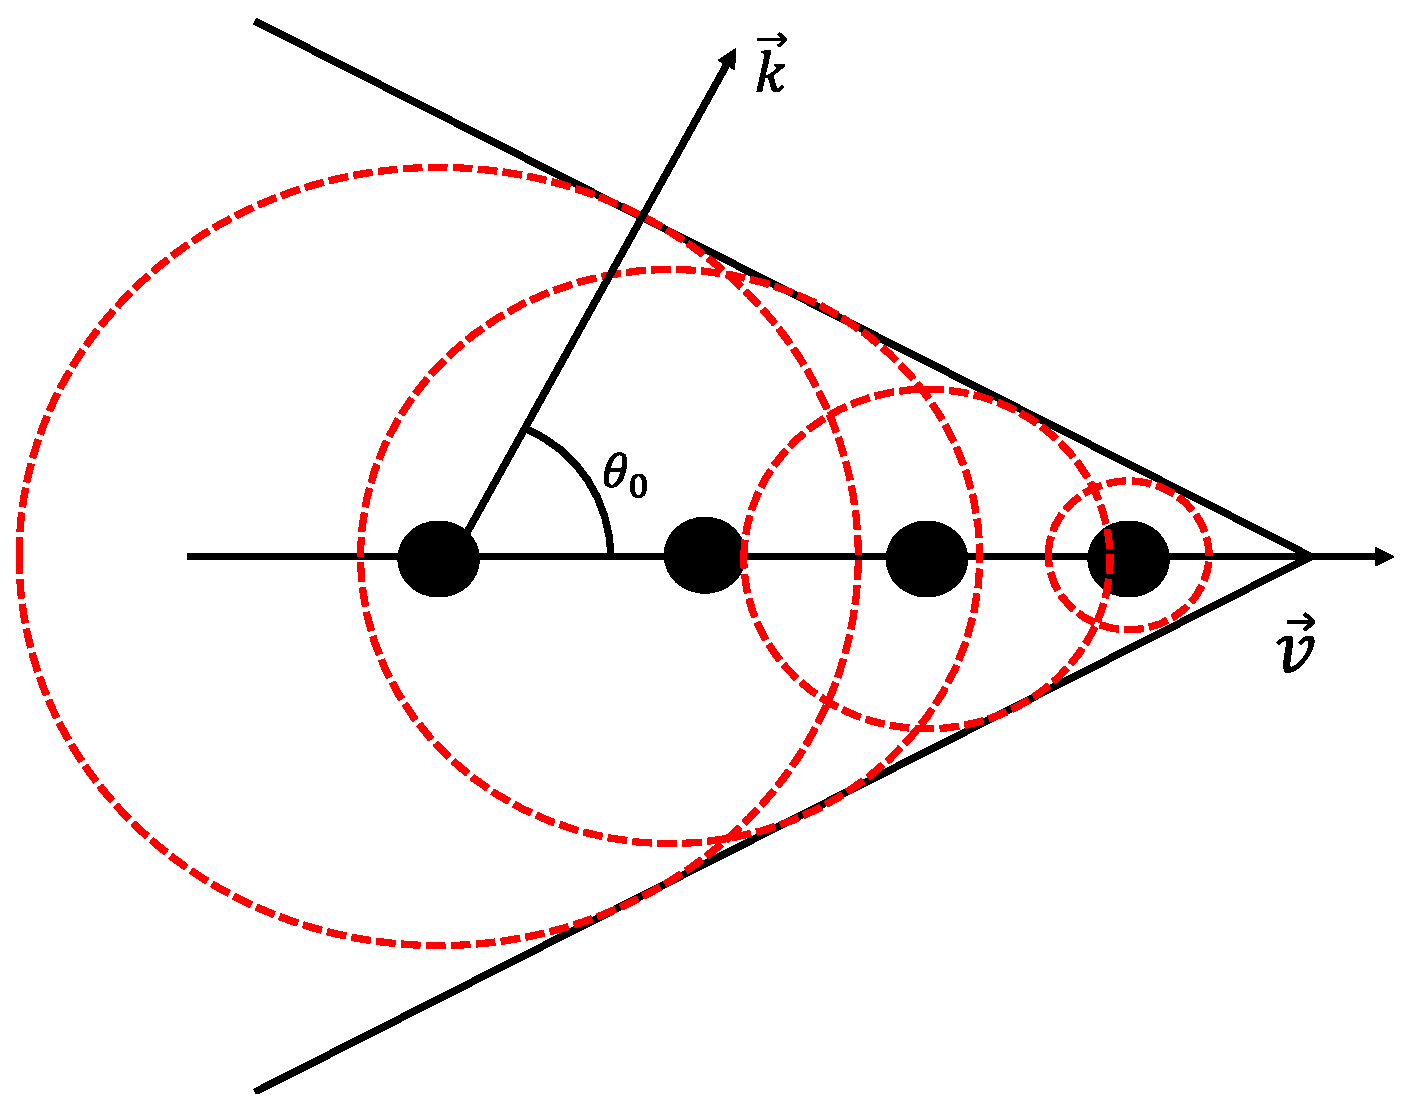
\includegraphics[width=0.4\textwidth]{Figure1.eps}% Here is how to import EPS art
\caption{\label{fig:cherenkov}Schematic diagram of Cherenkov Radiation. The black points stand for the snapshot of the electron at different times, the read dash circle refers to the current radiation surface from the previous electron.}
\end{figure}
% Adjust this value as needed
\begin{figure}
\centering
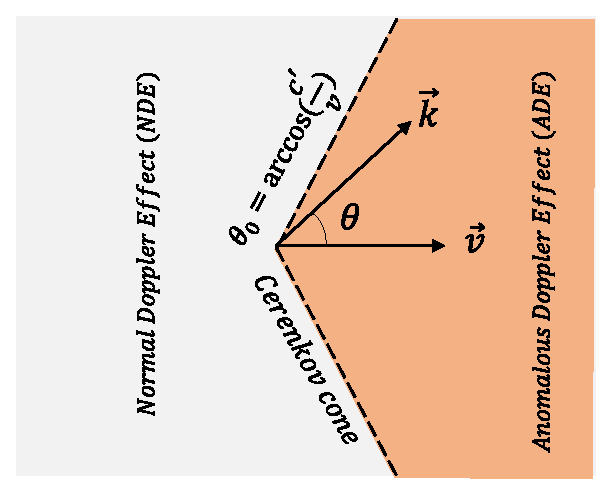
\includegraphics[width=0.4\textwidth]{Figure2.eps}% Here is how to import EPS art
\caption{\label{fig:ADENDE}The region of Anomalous Doppler Effect (ADE) and Normal Doppler Effect (NDE).}
\end{figure}

However, when the electron is replaced by a system possessing internal energy---such as an oscillator or a cyclotron electron in a magnetic field---the direction of the emitted photon is no longer determined by the interference of secondary waves and can instead occur in any direction. Considering a scenario where the system emits a photon with angular frequency $\omega$ and wavevector k, the emission process must satisfy both energy and momentum conservation:
\begin{subequations}
\begin{eqnarray}
T_1+U_1&=&\hbar \omega +T_2+U_2  \label{Tc} \\  
 \vec{p_1}&=&\vec{p_2}+\hbar\vec{k}   \label{Pc}
\end{eqnarray}
\end{subequations}

Here the T and U represent the kinetic energy and internal energy of the system while subscripts of 1 and 2 refer to before and after emitting a photon. p represents the momentum of the system and $\hbar$ represnts reduced Planck's constant. Assuming that photon’s energy is far less than the initial kinetic energy $T_1$, the losses of kinetic energy after emitting a photon can be expressed as $\Delta T_{12} = T_1 - T_2 = \Delta\vec{ p} \cdot \vec{v}$, where v is the velocity of the system before emitting a photon and $\Delta\vec{ p} = \vec{p}_1 - \vec{p}_2 = \hbar \vec{k}$. Thus, the change of internal energy can be expressed as 
\begin{equation} 
\begin{array}{rl}
\Delta U_{21} &= \Delta T_{12} - \hbar \omega \\
              &= \hbar \vec{k} \cdot \vec{v} - \hbar \omega \\
              &= \hbar \omega \left( \dfrac{v \cos \theta}{c'} - 1 \right)
\end{array} \label{eq:DeltaU00}
\end{equation}
Here, \(\omega / k = c'\), and \(\Delta U_{21} = U_2 - U_1\). When the system's velocity exceeds the speed of light in the medium (\(v > c'\)), the sign of \(\Delta U_{21}\) allows the radiation to be categorized into three distinct regions, as illustrated in Fig.~\ref{fig:ADENDE}.
\begin{enumerate}
\item For $\theta > \theta_0 = \arccos(c'/v)$, $\Delta U_{21} < 0$. The system produces photons by consuming its own internal and kinetic energy; this region refers to the Normal Doppler Effect (NDE).
\item For $\theta = \theta_0$, $\Delta U_{21} = 0$, the loss of kinetic energy by the system is completely converted into photon energy; this line refers to the Cerenkov Effect.
\item For $\theta < \theta_0$, $\Delta U_{21} > 0$, this region is referred to as the Anomalous Doppler Effect (ADE), where the system gains internal energy after emitting photons. It means the loss of kinetic energy is converted to photons and the system's internal energy.
\end{enumerate}
In previous paper, the change of internal energy is given as $\Delta U = m\hbar\omega_{ce}$, where $m = 0, \pm1, \pm2, \pm3, \ldots$ represent the Landau level, as given by V.\,L. Ginzburg~\cite{ginzburg2005radiation}, Coppi~\cite{coppi1976slide}, Frolov~\cite{frolov1986excitation}, Frank~\cite{frank1960optics}, Tamm~\cite{tamm1959general} and Nezlin~\cite{nezlin1976negative}. The above content revisits the foundational work of V.\,L. Ginzburg~\cite{ginzburg2005radiation}. In the present paper, it is further demonstrated that $m$ actually represents the quantum number associated with the angular momentum of the emitted photon.

Let's consider the process in which an electron cyclotron system under a uniform magnetic field emits a photon along z axis, as shown in Fig.~\ref{fig:Schematic}. The moving electron has the velocity $v_z$ along the background magnetic field and the $v_\perp$ cyclotron velocity. The kinetic energy along $z$ is $T = \gamma m_e c^2 - m_e c^2$, where $\gamma$ refers to the Lorentz factor. The internal energy represents as $U = \frac{1}{2} \gamma m_e v_\perp^2$. 

Assume the angular momentum of the system before and after emitting a photon is $L_1$ and $L_2$, respectively. The angular momentum of photon is $m\hbar$. According to the angular momentum conservation, we have
\begin{equation}
L_1 = L_2 + m\hbar \label{eq:AngularCon} 
\end{equation}

\begin{figure}
\centering
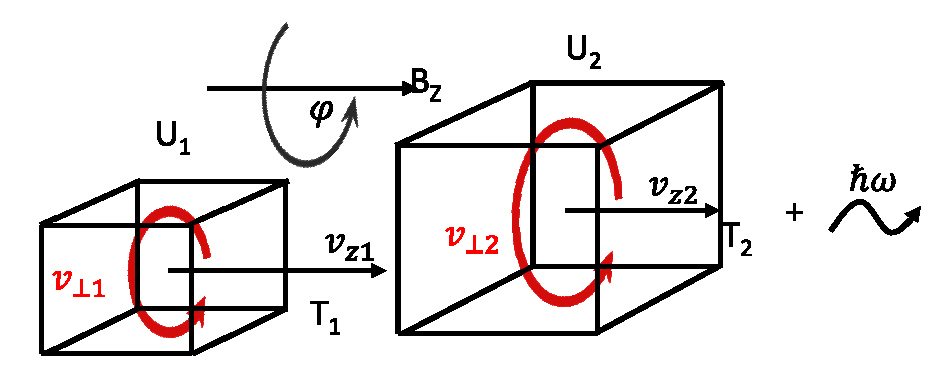
\includegraphics[width=0.7\textwidth]{Figure3.eps}% Here is how to import EPS art
\caption{\label{fig:Schematic}Schematic diagram of electron cyclotron system before and after emitting a photon. Here \(U_2>U_1, T_2<T_1\)}
\end{figure}


Since the magnetic field is aligned along z direction, the angular momentum of electron along z is represented as $L_z$. According to the quantum theory, the electron wave in the static magnetic field can be expressed as
\begin{equation}
\Psi = \Psi_0 e^{\frac{i}{\hbar} (\mathbf{p} - e\mathbf{A}) \cdot \mathbf{s}} \label{eq:psi}
\end{equation}
With the term $\Psi_0$ representing the normalized coefficient, $\mathbf{A}$ is the vector potential and $\mathbf{s}$ is the position. For a gyro-motion electron in a magnetic field, $\mathbf{s} = r\phi\,\vec{e}_\phi$, where $r$ refers to the cyclotron radius and $\phi$ refers to the cyclotron angle. 

The $z$-component of the orbital angular momentum operator can be expressed in spherical coordinates as:
\begin{equation}
\hat{L}_z = -i\hbar\frac{\partial}{\partial\phi}  \label{eq:Lz}
\end{equation}
Combining Eq.~(\ref{eq:psi}) with Eq.~(\ref{eq:Lz}), we have 
\begin{equation}
-i\hbar \frac{\partial}{\partial \phi} \Psi = (p_\phi - eA_\phi) r \Psi
\end{equation}
As a result, the eigenvalue of  $L_z $can be expressed as
\begin{equation}
L_z = (p_\phi - e A_\phi) r  \label{eq:Lz_2}
\end{equation}
With \( p_\phi = \gamma m_e v_\perp \), \( A_\phi = \dfrac{r B_0}{2} \), and \( r = \dfrac{\gamma m_0 v_\perp}{B_0 e} \), Eq.~(\ref{eq:Lz_2}) can be rewritten as:
\begin{equation}
L_z = \frac{1}{2} \cdot \frac{\gamma m_0 v_\perp^2}{\omega_{ce}} = \frac{U}{\omega_{ce}},
\end{equation}
where \(\omega_{ce} = \dfrac{eB}{m_0 \gamma} = \dfrac{\omega_0}{\gamma}\) and \(U = \dfrac{1}{2} \gamma m_0 v_\perp^2\).
Here, \( m_0 \) is the electron rest mass, \( \gamma \) is the Lorentz factor, and \( \omega_0 \) is the electron cyclotron frequency in the rest frame (\( here we choose \omega_0 > 0 \)). The conservation of angular momentum in the \( z \)-direction is expressed as
\[
L_{z2} + m\hbar = L_{z1}.
\]
The variation in the angular momentum of the electron along the \( z \)-axis is given by:
\begin{equation}
\Delta L_{21} = L_{z2} - L_{z1} = \frac{U_2 - U_1}{\omega_{ce}} = -m\hbar \label{eq:DeltaL21}
\end{equation}
Here, \( m \) is the quantum number of the photon's angular momentum in the \( z \)-direction. The internal energy change is given by \( \Delta U_{21} = U_2 - U_1 \). With Eq.~(\ref{eq:DeltaL21}), it can be transformed as:
\begin{equation}
\Delta U_{21}=-m \hbar \omega_{ce}  \label{eq:DeltaU21}
\end{equation}
According to the Eq.~(\ref{eq:DeltaU00})  and Eq.~(\ref{eq:DeltaU21}), the change in electron energy  could be presented as 
\begin{equation}
\hbar \vec{k} \cdot \vec{v} = \hbar \omega - m \hbar \omega_{ce} \label{eq:EnergyResonant}
\end{equation}
This result is consistent with previous findings~\cite{tamm1959general, frank1960optics, nezlin1976negative, coppi1976slide, frolov1986excitation, ginzburg1996radiation}. Here, \( \hbar \vec{k} \cdot \vec{v} \) represents the loss of kinetic energy \( \Delta T_{12} \), \( \hbar \omega \) represents the energy of the photon, and \( -m \hbar \omega_{ce} \) represents the change in the electron gyrokinetic energy \( \Delta U_{21} \) (the internal energy change). The ratio between the internal energy change \( \Delta U_{21} \) and the kinetic energy change \( \Delta T_{21} \) can be expressed as
\begin{equation}
\frac{\Delta U_{21}}{\Delta T_{21}} = \frac{m \hbar \omega_{ce}}{\hbar \vec{k} \cdot \vec{v}}  \label{eq:DU21DT21}
\end{equation}
 This results is a critical criterion to compare with the classical dynamic simulation in the section 2. It is also proved based on classical theory in the Appendix.
After simpifying the Eq.~(\ref{eq:EnergyResonant}), we finally have the classical wave-particle resonant condition 
\begin{equation}
\omega = k_z v_z + m \omega_{ce}
\end{equation}
The variable \( m \) represents the quantum number associated with the angular momentum of the photon. Since a photon possesses both orbital angular momentum (\( l\hbar\), where \(l = 0,\pm1,\pm2,\pm3,... \)) and intrinsic spin angular momentum (\( s\hbar \), where \( s = \pm 1 \))~\cite{arnaut2000orbital}, the total angular momentum can be expressed as \( m\hbar = l\hbar + s\hbar \). 

For photons carrying only spin angular momentum, two distinct quantum states are possible, characterized by the spin quantum number $m$:

\begin{enumerate}
\item For $m=+1$ ($\Delta U_{21}<0$), the cyclotron electron loses internal energy upon photon emission. The emitted photon displays right-hand circular polarization . This process is known as the NDE. 

\item For $m=-1$ ($\Delta U_{21}>0$), the cyclotron electron gains internal energy through photon emission. The emitted photon exhibits left-hand circular polarization \footnote{The difference between our definition of circular polarization and the standard definition~\cite{kiang2008angular} stems from our choice of $\omega_0 > 0$. Here, $m > 0$ corresponds to the same rotational sense as the electron's natural right-hand gyration, which yields right-hand polarization when $\vec{k} \parallel \vec{B}_0$.}. This process corresponds to the ADE.
\end{enumerate}


%above describe spontaneous emission phenomenon of ADE and NDE without external field intervention . In our simulation model , an external plane EM field is introduced as resonant field interacting with electrons . the plane EM wave actually play a role as induced wave, where gyro-electron may absorb or stimulated em wave. from quantum from, the plane em wave actually is the ocean of photon which only contains spin angular momentum. so we should get the same resonant condition as derived from quantum field , where the righ hand polarization wave corresponds to $m = 1$ \cite{wei2024spin} and could only resonant under condition $\omega=\omega_c{e}+\vec{k}\cdot\vec{v}$,which is corresponds to NDR, while left-hand polarization corresponds to $m=-1$ and could only resonant with electron under $\omega=-\omega_{ce}+\vec{k}\cdot\vec{v}$,which is correspond to ADR
The above discussion described spontaneous emission phenomena of ADE and NDE without external field intervention. In our simulation model, we introduce an external plane electromagnetic (EM) wave that serves as a resonant field interacting with electrons. This plane EM wave acts as an inducing field, enabling gyro-electron to undergo stimulated absorption or emission processes. 
From a quantum perspective,  the plane EM wave can be regarded as an ocean of photons that carry only spin angular momentum. Consequently, the same resonance conditions as those derived from quantum field theory are recovered:

\begin{itemize}
    \item Right-hand circularly polarized  waves correspond to $m = +1$ states \cite{wei2024spin}, resonating only when $\omega = \omega_{ce} + \vec{k}\cdot\vec{v}$ (NDR condition)
    
    \item Left-hand circularly polarized  waves correspond to $m = -1$ states, resonating only when $\omega = -\omega_{ce} + \vec{k}\cdot\vec{v}$ (ADR condition)
\end{itemize}

This exact correspondence between our classical simulation framework and quantum field theoretic predictions validates our modeling approach while providing physical insight into the angular momentum selection rules governing these resonant interactions.


Although nonlinear analyses of electron interactions with electromagnetic waves have been extensively studied \cite{liu2004particle,qian1999exact,weyssow1990motion,gogoberidze2005origin,roberts1964motion,bourdier2000dynamics,nusinovich1999theory,nusinovich1995theory,qian2000relativistic}, the specific role of static electric fields in these interactions has received comparatively less attention. In our approach, the uniform electric field serves a crucial function by systematically scanning the electron velocity, thereby enabling investigation across the full spectrum of resonance conditions. The inherent complexity of these nonlinear processes precludes analytical solutions, necessitating the use of numerical simulation methods to obtain meaningful physical insights.

\section{Classical dynamic simulation of ADR}\label{sec:level3}
The ADE process has been analyzed based on quantum theory, demonstrating that the angular momentum of the emitting photon determines the resonance condition.  These characteristics will be tested through the interaction of EM wave and the electron during ADR and NDR, and the energy transfer ratio can also be verified through numerical simulations.
\subsection{Numerical simulation setup}
To analyze the resonant process from the perspective of classical dynamics and to provide a direct comparison between quantum and classical dynamic results, the following scenario is considered: A uniform magnetic field \( \vec{B}_0 \) is applied along the \( z \)-direction. An electrostatic field \( \vec{E}_0 \), oriented in the opposite direction to \( \vec{B}_0 \) (as illustrated in Fig.~\ref{fig:Setup}), is used to accelerate the electron. 
\begin{figure}
\centering
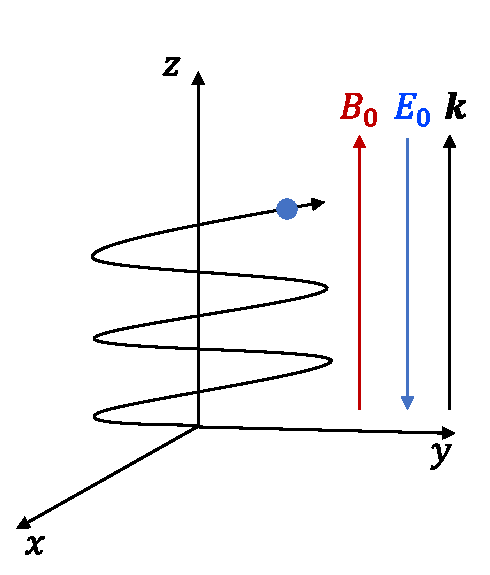
\includegraphics[width=0.4\textwidth]{Figure4.eps}% Here is how to import EPS art
\caption{\label{fig:Setup}The uniform static magnetic field is set along the z axis, the electrostatic field $E_0$ is oriented opposite to the $B_0$ field, and the wavevector $k$ is aligned parallel to the $B_0$ field.}
\end{figure}
We consider the interaction between an electron entering the system with velocity \( v_z \), parallel to the magnetic field \( B_0 = B_z \), and a linearly or circularly polarized transverse electromagnetic (TEM) wave propagating in a homogeneous dielectric medium with a refractive index \( n > 1 \).

The induced linearly polarized wave along \( \vec{B}_0 \) can be decomposed into a combination of a right-hand circularly polarized wave (\( m = 1 \)) and a left-hand circularly polarized wave (\( m = -1 \)), such that
\(
\vec{E}_w = \vec{E}_R + \vec{E}_L,
\)
where
\(
\vec{E}_R = \frac{1}{2} E_0 (\vec{e}_x + i\vec{e}_y) \exp[i(\vec{k} \cdot \vec{r} - \omega t)],
\vec{E}_L = \frac{1}{2} E_0 (\vec{e}_x - i\vec{e}_y) \exp[i(\vec{k} \cdot \vec{r} - \omega t)].
\)
%If the wavevector \( \vec{k} \) lies in the \( y \)-\( z \) plane with a crossing angle \( \theta_k \) relative to the \( z \)-axis, then the new coordinate unit vectors for the wave field expression should be rotated accordingly to align with the direction of \( \vec{k} \). The transformed basis vectors are:
%\begin{equation}
%\begin{pmatrix}
%\vec{e}_x' \\
%\vec{e}_y'
%\end{pmatrix}
%=
%\begin{pmatrix}
%1 & 0 & 0 \\
%0 & \cos\theta_k & \sin\theta_k
%\end{pmatrix}
%\cdot
%\begin{pmatrix}
%\vec{e}_x \\
%\vec{e}_y \\
%\vec{e}_z
%\end{pmatrix}
%\end{equation}
The magnetic field of E.M wave is
\begin{equation}
\vec{B}_w = \frac{\vec{k} \times \vec{E}_w}{\omega}
\end{equation}

The six-dimensional phase space of an electron, described by its position $\bm{r}$ and momentum $\bm{p}$, are presented in the equations below. The vectors $\bm{E}$ and $\bm{B}$ represent the total field, including both static and electromagnetic components. Here, $c$ denotes the speed of light in vacuum, $e$ represents the electron’s charge and $m_0$ is the electron’s mass in the rest frame.

\begin{equation}
\begin{aligned}
\frac{d\bm{r}}{dt} &= \frac{\bm{p}}{\sqrt{m_0^2 + \frac{\bm{p}^2}{c^2}}}, \\
\frac{d\bm{p}}{dt} &= -e \left( \bm{E}(\bm{r}, t) + \frac{\bm{p}}{\sqrt{m_0^2 + \frac{\bm{p}^2}{c^2}}} \times \bm{B}(\bm{r}, t) \right)
\end{aligned}
\end{equation}

To simulate the evolution of $\bm{r}$ and $\bm{p}$, the above system is discretized using the Volume-Preserving Algorithm. Let $j$ denote the iteration step and $\text{Cay}(\bm{A})$ represent the Cayley transform of matrix $\bm{A}$:

\begin{equation}
\left\{
\begin{aligned}
\bm{r}^*_{j+\frac{1}{2}} &= \bm{r}^*_j + \frac{\Delta t^*}{2 \gamma_j} \bm{p}^*_j, \\
\bm{p}^{*-} &= \bm{p}^*_j + \frac{\Delta t^*}{2} \bm{E}^*_{j+\frac{1}{2}}, \\
\bm{p}^{*+} &= \text{Cay} \left( \frac{\Delta t^* \hat{\bm{B}}^*}{2 \gamma^{*-}} \right) \bm{p}^{*-}, \\
\bm{p}^*_{j+1} &= \bm{p}^{*+} + \frac{\Delta t^*}{2} \bm{E}^*_{j+\frac{1}{2}}, \\
\bm{r}^*_{j+1} &= \bm{r}^*_{j+\frac{1}{2}} + \frac{\Delta t^*}{2 \gamma_{j+1}} \bm{p}^*_{j+1},
\end{aligned}
\right.
\end{equation}
The dimensionless parameters are momentum \( p^* = p/(m_0 c) \), magnetic field \( B^* = B/(e \tau_{ce} m_0) \), total electric field \( E^* = E/(\frac{m_0 c}{\tau_{ce} e}) \), time step \( \Delta t^* = \Delta t / \tau_{ce} \), and position \( r^* = r / (\tau_{ce} c) \) respectively, where the \( \tau_{ce} \) is the electron cyclotron period (\( \tau_{ce} = 2\pi / \omega_{ce} \)) and \( \gamma^* = \sqrt{1 + p^{*2}} \) is Lorentz factor. The dimensionless magnetic matrix \( \mathbf{B}^* \) \cite{zhang2015volume} is written as

\begin{equation}
\hat{B}^* =
\begin{pmatrix}
0 & B_z^* & -B_y^* \\
-B_z^* & 0 & B_x^* \\
B_y^* & -B_x^* & 0
\end{pmatrix}
\end{equation}
To illustrate the system evolution, the parameters are set as following: background magnetic field \( B_0 = 0.02\,T \), wave angular frequency \( \omega_s = 1.5 \omega_0 \) where \( \omega_0 = (e B_0)/m_0 \), wavevector \( \vec{k} = 10^5/\mathrm{m} \), the electric field component of the electromagnetic wave \( E_w = 9\,\mathrm{V/m} \). The propagation of induced wave with linear polarization is parallel to z axis, and the electrostatic field is \( E_0 = -2.5\,\mathrm{V} \). The time resolution is always chosen to satisfy 
\(
\Delta t = \min \left( \frac{2\pi}{50(\vec{k} \cdot \vec{v})}, \frac{2\pi}{50\omega_0}, \frac{2\pi}{(50\omega_0)} \right)
\)
to ensure the accuracy of the simulation.

\vspace{1em}

The evolution of the electron’s motion is shown in Fig.~\ref{fig:kinetic_evolution}. As the electron accelerates from stationary in the electrostatic field (Fig.~\ref{fig:kinetic_evolution}(b)), the resonant frequencies increase simultaneously (Fig.~\ref{fig:kinetic_evolution}(a)). The change of parallel velocity caused by electromagnetic wave can be quantified as \( \Delta v = v_z - v_{zE0} \) as shown in Fig.~\ref{fig:kinetic_evolution}(c), where \( v_z \) represents the parallel velocity under the given scenario, while \( v_{zE0} \) denotes the parallel velocity resulting solely from the electrostatic field, which can be calculated using a theoretical equation as

\begin{equation}
v_{zE0} = \frac{e E_0 t}{m_0 \sqrt{1 + \left( \frac{e E_0 t}{m_0 c} \right)^2 }}
\end{equation}

\vspace{1em}

The cyclotron velocity is shown in Fig.~\ref{fig:kinetic_evolution}(d). The work done by electromagnetic wave is shown in fig. 5(e), which can be calculated by integrating the power with time as 
\(
E_{\parallel \text{emw}} = \int P_{\parallel \text{emw}} dt ,
\)
and 
\(
P_{\parallel \text{emw}} = -e \vec{v}_\perp \times \vec{B}_{\perp \text{emw}} \cdot v_z.
\)
Since all discrete data points are available from the simulation, it is not difficult to integrate all the discrete data over time. Fig.~\ref{fig:kinetic_evolution}(f) shows the gyro-kinetic energy evolution with time, where 
\(
E_\perp = \frac{1}{2} m_e v_\perp^2.
\)

\begin{figure}[ht]
\centering
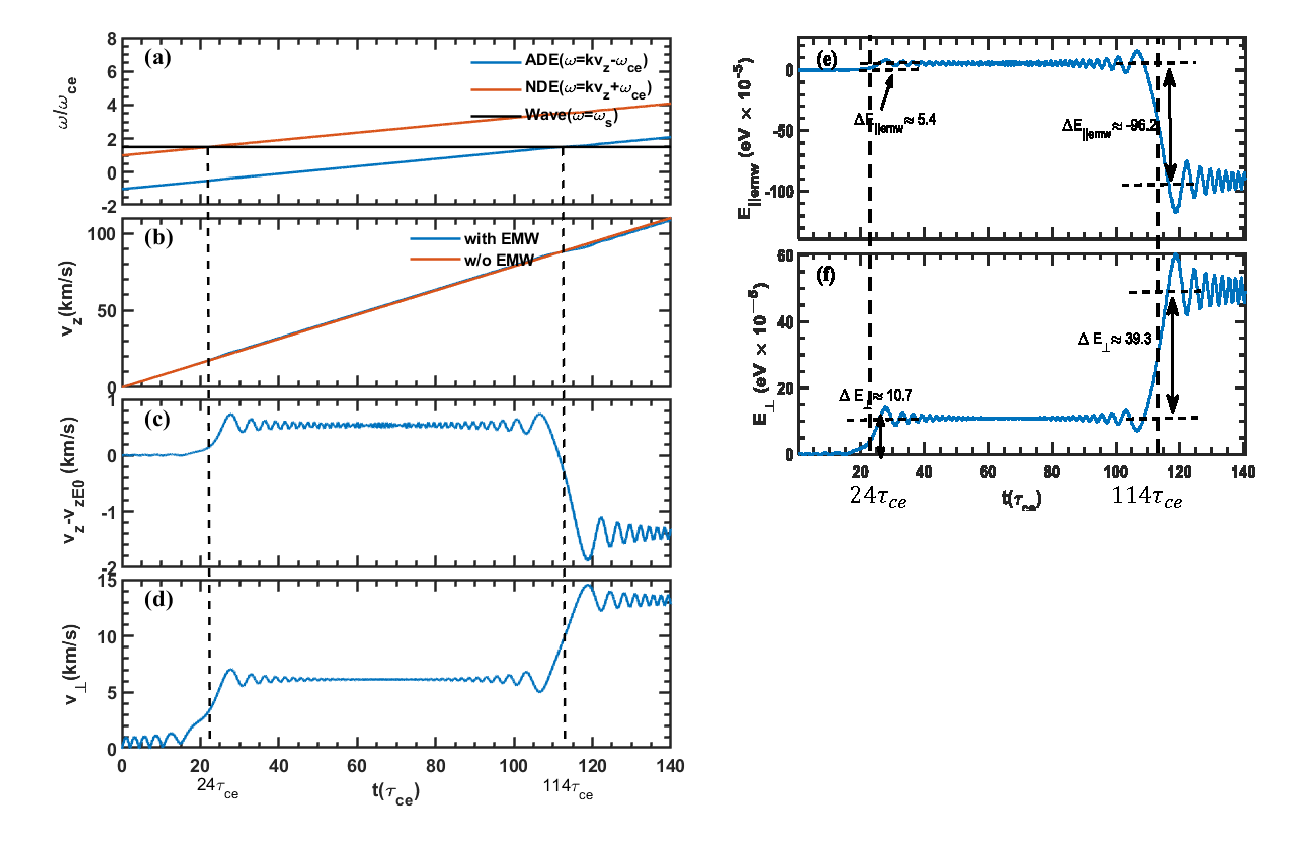
\includegraphics[width=0.8\textwidth]{Figure5.pdf}% Here is how to import EPS art
\caption{\label{fig:NumSim}Kinetic evolution of electrons in a magnetic field with an electromagnetic wave during acceleration. 
    (a) Frequencies of ADE, NDE, and source wave frequency. 
    (b) The parallel velocity $v_z$ in the case with and without the electromagnetic wave. 
    (c) The change of parallel velocity caused by the electromagnetic wave. 
    (d) The cyclotron velocity $v_\perp$. 
    (e) The parallel kinetic energy transferred to the electron by the electromagnetic wave. 
    (f) The evolution of gyro-kinetic energy.}
    \label{fig:kinetic_evolution}
\end{figure}


\subsection{Validation of energy transfer ratio  }

As shown in Fig.~\ref{fig:kinetic_evolution}(a), around \( 23\tau_{ce} \), the normal doppler frequency matches that of the induced wave, leading to a rapid increase in the cyclotron velocity \( v_{\perp} \) (Fig.~5(b)). Simultaneously, the change in parallel velocity induced by the electromagnetic wave also increases. This phenomenon can be interpreted as the electron cyclotron system absorbing a photon during the NDR, resulting in an increase in both parallel kinetic energy and gyro-kinetic energy(internal energy). The change in parallel kinetic energy caused by the electromagnetic wave is shown in Fig.~\ref{fig:kinetic_evolution}(e), where \( \Delta T_{21} = \Delta E_{||\text{emw}} \approx 5.4 \times 10^{-5} \, \text{eV} \). The increase in gyro-kinetic energy is shown in Fig.~\ref{fig:kinetic_evolution}(e), where \( \Delta U_{21} = \Delta E_{\perp} \approx 10.7 \times 10^{-5} \, \text{eV} \). The energy transfer ratio between internal energy and parallel kinetic energy during resonance is given by \( \frac{\Delta U_{21}}{\Delta T_{21}} \approx 1.98 \). According to quantum theory, the energy ratio is given by Eq.~(13). Here \( m = 1 \) for NDE and \( k = 10^5 \, \text{m}^{-1} \) along the \( z \)-axis, the resonant velocity \( v_z \approx 19 \times 10^3 \, \text{m/s} \) and \( \omega_{ce} \approx 3.51 \times 10^9 \, \text{s}^{-1} \). Finally, \( n_p = 1.85 \), which is in close agreement with the simulation results.

The Anomalous Doppler Effect begins to emerge when the time reaches \( 113 \tau_{ce} \), where \( \omega_{\text{ADE}} = \omega \) as shown in Fig.~\ref{fig:kinetic_evolution}(a). At this point, the parallel velocity begins to scatter into the perpendicular direction, evident from the decrease in \( \Delta v_z \) and the increase in \( v_{\perp} \) as seen in Fig.~\ref{fig:kinetic_evolution}(c) and Fig.~\ref{fig:kinetic_evolution}(d). During the resonant period, the changes in parallel kinetic and gyro-kinetic energies caused by the electromagnetic wave are calculated as \( \Delta T_{21} = \Delta E_{||\text{emw}} \approx -96.2 \times 10^{-5} \, \text{eV} \) and \( \Delta E_{\perp} \approx 39.3 \times 10^{-5} \, \text{eV} \). The energy transfer ratio is \( \frac{\Delta U_{21}}{\Delta T_{21}} \approx -0.408 \). According to quantum theory, the change ratio of \( \Delta U_{21}/\Delta T_{21} = -\hbar \omega_{ce}/\hbar \vec{k} \cdot \vec{v} = -0.3908 \), where \( \omega_{ce} \approx 3.51 \times 10^9 \, \text{s}^{-1} \), and \( k = 10^5 \, \text{m}^{-1} \), \( v_z = 90 \, \text{km/s} \). The quantum theory results are in good agreement with the numerical calculations. The energy change ratio is also derived in the Appendix, based on classical theory.
\subsection{Validation of the relationship with wave angular momentum. }
\begin{figure}[ht]
\centering
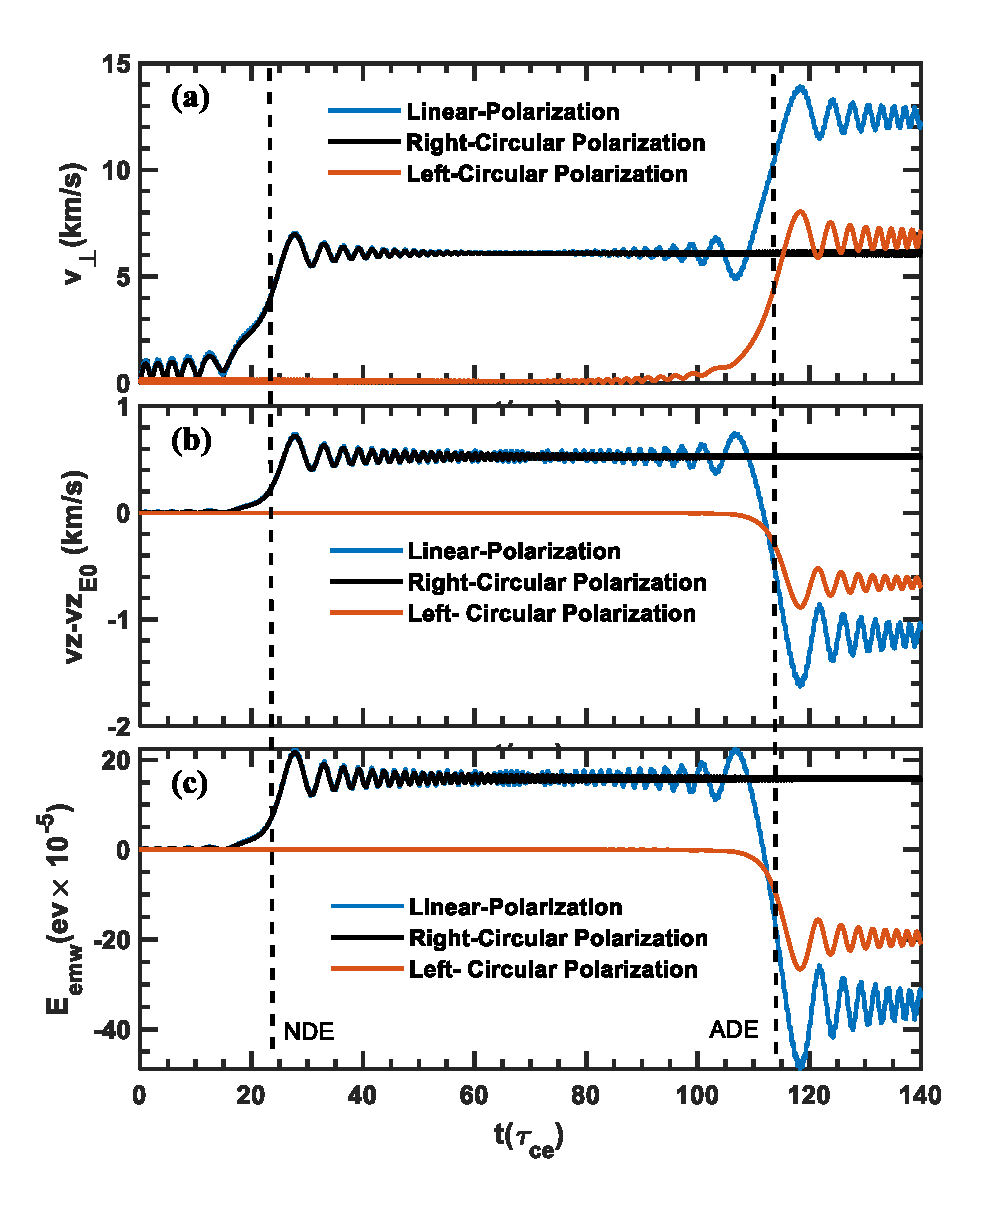
\includegraphics[width=0.5\textwidth]{Figure6.eps}% Here is how to import EPS art
\caption{Velocity evolution caused by induced wave with linear, right-circular and left-circular polarization. (a) The cyclotron velocity $v_\perp$ .(b) The change of parallel velocity caused by the electromagnetic wave.}
    \label{fig:AngularMomentum}
\end{figure}

Fig.~\ref{fig:AngularMomentum}(a--b) illustrate the velocity evolution under linear polarization of \( E_l \), right-circular polarization \( E_R \) (\( m = -1 \)), and left-circular polarization \( E_L \) (\( m = 1 \)). The work done on the electron by the electromagnetic wave, \( E_{\text{emw}} \), as depicted in Fig.~\ref{fig:AngularMomentum}(c), consists of the parallel direction, \( E_{\parallel\text{emw}} \), as previously described, and the gyro-kinetic energy \( E_{\perp\text{emw}} \). The latter is calculated as
\(
E_{\perp\text{emw}} = \int \vec{F}_{\perp} \cdot \vec{v}_{\perp} \, dt,
\)
where \( \vec{F}_{\perp} \) is determined from the electric and magnetic field forces, and \( \vec{v}_{\perp} \) represents the cyclotron velocity. All these parameters can be readily obtained from numerical results and integrated discretely.

The three types of polarization waves are investigated under the same scenario as before. As a result, the right-hand circularly polarized wave (\( m = 1 \)) causes a velocity change only at around \( 23\tau_{ce} \), while the left-hand circularly polarized wave (\( m = -1 \)) causes a velocity change only at around \( 113\tau_{ce} \). This indicates that the right-circularly polarized wave is responsible for the NDE, while the left-hand circularly polarized wave is responsible for the ADE, which agrees well with the quantum analysis.

%The process can be understood as follows: For an electromagnetic wave with right-hand polarization propagating along the magnetic field, the electron in the magnetic field undergoes right-hand circular motion. When its parallel velocity satisfies the condition
%\(
%\omega - \vec{k} \cdot \vec{v} = \omega_{ce},
%\)
%known as the Normal Doppler Resonance (NDR) condition, the electron, in its co-moving cyclotron frame, perceives the wave frequency as equal to its rotational frequency. Consequently, the electron resonates and absorbs the electromagnetic wave, as indicated in Fig.~\ref{fig:AngularMomentum}(c) at \( 23\tau_{ce} \). According to the conservation of angular momentum and parallel momentum, both the cyclotron velocity and parallel velocity increase, as the electromagnetic wave carries positive angular momentum (in the same direction as the cyclotron electron's angular momentum) and parallel momentum, which correspond to \( \hbar \) and \( \hbar k \) in quantum physics.
%
%For a left-circularly polarized electromagnetic wave, the resonance and scattering process occurs when the electron velocity satisfies the condition
%\(
%\omega - \vec{k} \cdot \vec{v} = -\omega_{ce},
%\)
%known as the ADR. In the frame of the cyclotron electron, the electromagnetic wave has the same frequency and rotational direction as the electron, since the electron's velocity exceeds the wave phase velocity. Because the electromagnetic wave performs negative work on the electron, as shown in Fig.~\ref{fig:AngularMomentum}(c) at \( 113\tau_{ce} \), where \( E_{\text{emw}} \) is negative for a left-hand polarization wave, this is equivalent to the electron emitting an electromagnetic wave with the same properties as the induced wave. Since the emitted wave has left-hand circular polarization and positive momentum---corresponding to \( -\hbar \) and \( \hbar k \) in quantum physics---the cyclotron velocity increases while the parallel velocity decreases, to conserve angular momentum and momentum.
%
%For the left-circularly polarized wave, where the angular momentum \( m = -1 \), resonance occurs only at
%\(
%\omega = \vec{k} \cdot \vec{v} - \omega_{ce},
%\)
%as shown in Fig.~\ref{fig:7}. This behavior differs from previous results, where resonance for a plane electromagnetic wave could occur at any integer \( m \) satisfying
%\(
%\vec{k} \cdot \vec{v} + m\omega_{ce} - \omega = 0,
%\)
%as shown in Eq.~(36) and Eq.~(37) of Ref.~\cite{dendy1987classical}, but agrees well with angular momentum conservation analysis.
For a left-circularly polarized (LCP) electromagnetic wave, The angular momentum selection rule ($m = -1$) restricts resonance to only occur when:
\(
    \omega = \vec{k} \cdot \vec{v} - \omega_{ce},
\)
as confirmed numerically in Fig.~\ref{fig:7}. This represents a significant departure from previous classical treatments \cite{dendy1987classical} (Eqs. 36-37) that permitted resonance at arbitrary integer harmonics $m$, while being fully consistent with quantum angular momentum conservation principles.



\begin{figure}[htbp]
\centering
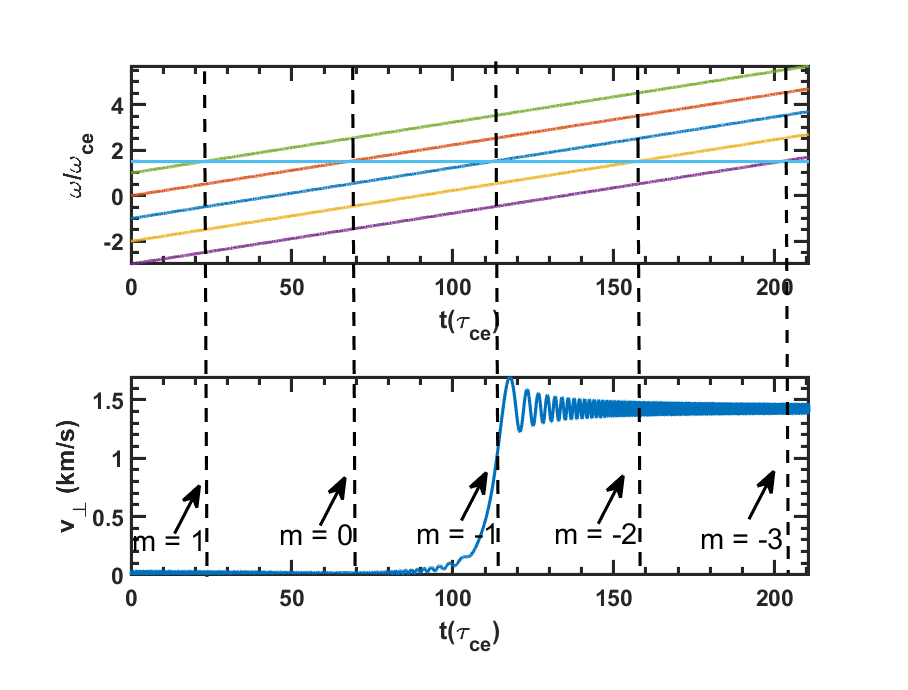
\includegraphics[width=0.8\textwidth]{Figure7.eps}% Here is how to import EPS art
\caption{\label{fig:7}(a) Frequency of $\omega = \vec{k} \cdot \vec{v} + m\omega_{ce}$ under different $m$ values and induced wave frequencies.(b)Perpendicular velocity evolution under the left-circularly polarized wave, where $m = -1$.}
\end{figure}





\section{Discussion }\label{sec:Discussion}
Based on the momentum and angular momentum conservation analysis, we analyze the case where $\vec{k}$ is oriented opposite to $v_{\parallel}$(or $\vec{B_0}$). In this case, if a cyclotron electron emits a photon with left-hand circular polarization and momentum $-\hbar\vec{k}$, where the angular momentum carried by photon is $\hbar$, then after the emission, the change in internal energy is $\Delta U = -\hbar\omega_{ce}<0$, and the change in translational kinetic energy $\Delta T = \hbar k v_{\parallel}>0$. However, if the emitting photon have right-circular polarization and momentum $-\hbar\vec{k}$, the change of internal energy becomes $\Delta U = \hbar\omega_{ce}>0$, while the translational kinetic energy still is $\Delta T = \hbar k v_{\parallel}>0$. This would violate the conservation of energy, as it is not possible for an electron to emit a photon while simultaneously increasing its total energy. Consequently, for a plane electromagnetic wave, only the left-circularly polarized component can resonate with an electron moving opposite to $v_{\parallel}$ (or $\vec{B_0}$). 
%Based on momentum and angular momentum conservation analysis, we examine the case where $\vec{k}$ is oriented opposite to $\vec{v}_{\parallel}$ (or $\vec{B_0}$). 
%\begin{itemize}
%    \item \textbf{Left-hand circular polarization case}: When a cyclotron electron emits a photon with:
%
%    \begin{itemize}
%        \item Left-hand circular polarization ($\sigma^-$)
%        \item Momentum $-\hbar\vec{k}$
%        \item Angular momentum $+\hbar$
%    \end{itemize}
%    the resulting energy changes are:
%    \begin{align}
%        \Delta U &= -\hbar\omega_{ce} < 0 \quad \text{(decrease in internal energy)} \\
%        \Delta T &= +\hbar k v_{\parallel} > 0 \quad \text{(increase in translational energy)}
%    \end{align}
%
%    \item \textbf{Right-hand circular polarization case}: If the emitted photon had:
%    \begin{itemize}
%        \item Right-hand polarization ($\sigma^+$)
%        \item Momentum $-\hbar\vec{k}$
%        \item Angular momentum $-\hbar$
%    \end{itemize}
%    the energy changes would instead be:
%    \begin{align}
%        \Delta U &= +\hbar\omega_{ce} > 0 \quad \text{(increase in internal energy)} \\
%        \Delta T &= +\hbar k v_{\parallel} > 0 \quad \text{(increase in translational energy)}
%    \end{align}
%\end{itemize}

The right-hand polarization case would violate energy conservation, as it requires the electron to \emph{emit} a photon while simultaneously \emph{gaining} total energy ($\Delta U + \Delta T > 0$). 
Therefore, for a plane electromagnetic wave, only the left-circularly polarized component can resonantly interact with an electron moving antiparallel to $\vec{v}_{\parallel}$ while satisfying all conservation laws.



\section{Conclusion}\label{sec:Conclusion}
This paper presents a simple yet useful method to analyze the resonant process of NDE and ADE. The quantum method, combined with an angular momentum conservation analysis, illustrates that the parameter $m$ in the resonant condition $\omega = \vec{k} \cdot \vec{v} + m\omega_{ce}$ is directly related to the angular momentum of the resonant wave. Numerical simulations based on the VPA method are also provided, confirming the correctness of the quantum results regarding both the angular momentum relationship between $m$ and the energy transfer ratio.

%\addcontentsline{toc}{chapter}{Appendix A: Appendix section heading}
\section*{Appendix A:Classical analysis of Anomalous Doppler Resonant}
here we would like give a brief derivation of energy transformation through classical dynamic equation:
\begin{align}
m_e \frac{d\vec{v}_\parallel}{dt} &= -e(\vec{v}_\perp \times \vec{B}_\perp) \label{eq:19} \\
m_e \frac{d\vec{v}_\perp}{dt} &= -e(\vec{v}_\perp \times \vec{B}_0 + \vec{v}_\parallel \times \vec{B}_\perp + \vec{v}_\perp \times \vec{B}_0) \label{eq:20}
\end{align}

Consider $\vec{B}_\perp = \frac{\vec{e}_k \times \vec{E}_\perp}{v_p}$, where $\vec{e}_k$ is the unit vector of wave vector of E.M. wave, which is along the $z$-axis. Using $\vec{v}_\parallel$ and $\vec{v}_\perp$ to dot both sides of \eqref{eq:19} and \eqref{eq:20}, substitute $\vec{B}_\perp$ and simplify the equations, we have

\begin{align}
m_e \vec{v}_\parallel \cdot \frac{d\vec{v}_\parallel}{dt} &= -e(\vec{v}_\perp \cdot \vec{E}_\perp) \frac{v_\parallel}{v_p} \label{eq:21} \\
m_e \vec{v}_\perp \cdot \frac{d\vec{v}_\perp}{dt} &= e(\vec{v}_\perp \cdot \vec{E}_\perp) \frac{v_\parallel}{v_p} - e(\vec{v}_\perp \cdot \vec{E}_\perp) \label{eq:22}
\end{align}

Here $v_p = \frac{\omega}{\kappa}$, the total energy change of electron can be expressed as:

\begin{equation}
\frac{d}{dt} \left( \frac{1}{2} m_e v_\parallel^2 + \frac{1}{2} m_e v_\perp^2 \right) = -e(\vec{v}_\perp \cdot \vec{E}_\perp) \label{eq:23}
\end{equation}

The sign of $-e(\vec{v}_\perp \cdot \vec{E}_\perp)$ determines whether the electromagnetic (E.M.) wave undergoes ``emission'' ($-e(\vec{v}_\perp \cdot \vec{E}_\perp) < 0$) or ``absorption'' ($-e(\vec{v}_\perp \cdot \vec{E}_\perp) > 0$) of E.M. wave, and this is dependent on the phase difference between $v_\perp$ and $E_\perp$.

From \eqref{eq:22} we have

\begin{equation}
e(\vec{v}_\perp \cdot \vec{E}_\perp) = \frac{m_e \vec{v}_\perp \cdot \frac{d\vec{v}_\perp}{dt}}{v_\parallel - 1} \label{eq:24}
\end{equation}

Substitute \eqref{eq:24} into \eqref{eq:21}, we have

\begin{equation}
m_e \vec{v}_\parallel \cdot \frac{d\vec{v}_\parallel}{dt} = -\frac{m_e \vec{v}_\perp \cdot \frac{d\vec{v}_\perp}{dt}}{v_\parallel - 1} \frac{v_\parallel}{v_p} \label{eq:25}
\end{equation}

Integrate \eqref{eq:25}, we have
\begin{equation}
\frac{1}{2}\,m_{\varrho}\left(v_{1}-\frac{\omega}{k}\right)^{2}+\frac{1}{2}\,m_{\varrho}v_{\perp}^{2}=C_{0}
\label{eq:26}
\end{equation}
\begin{figure}[htbp]
\centering
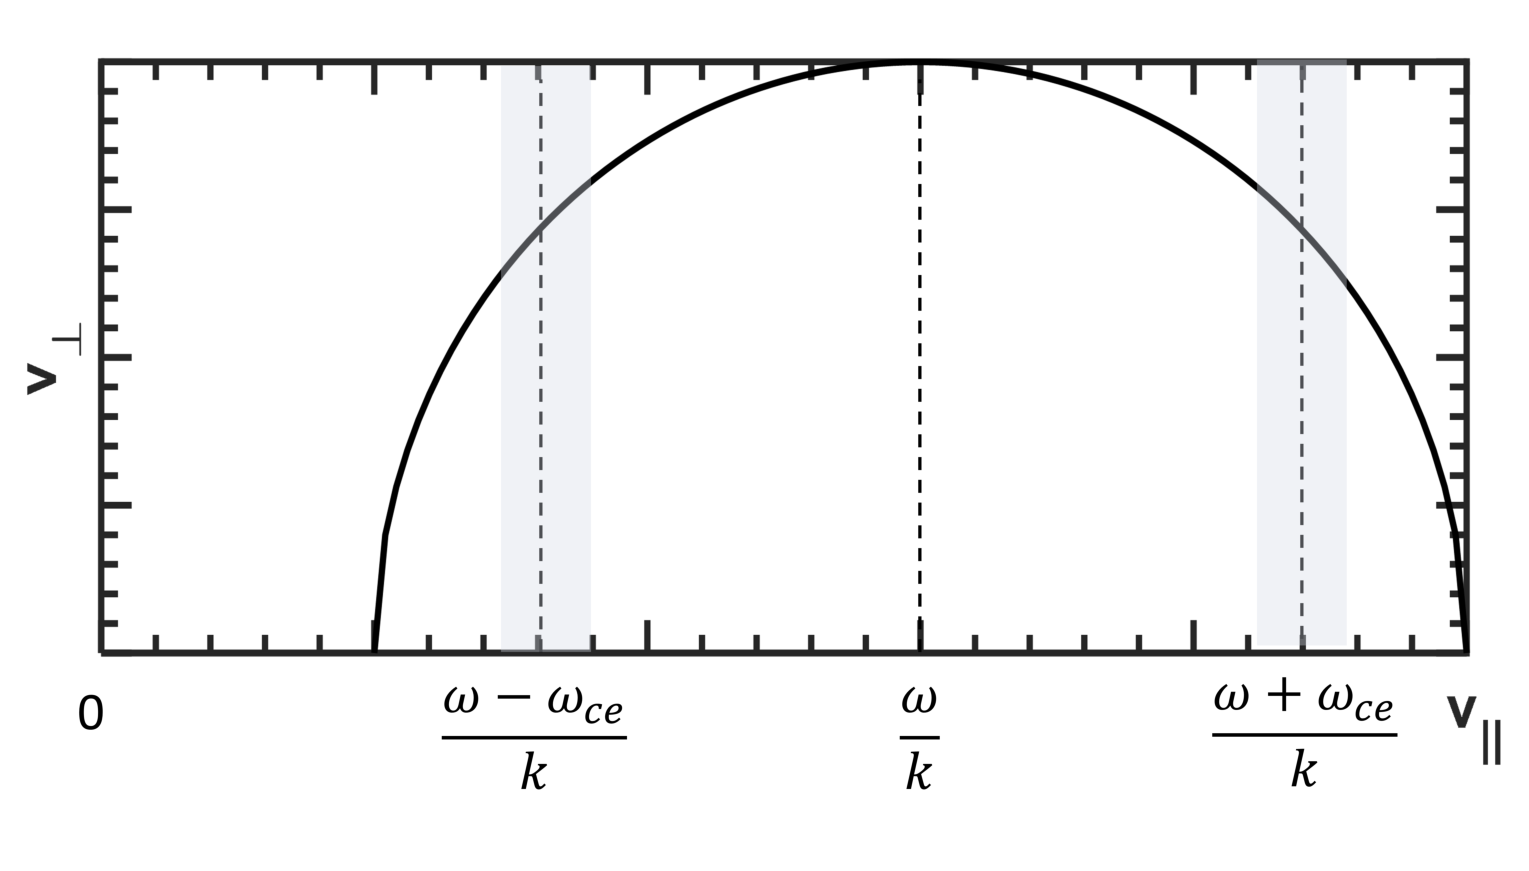
\includegraphics[width=0.8\textwidth]{Figure8.eps}% Here is how to import EPS art
\caption{\label{fig:8}The trajectory curve of $ (v_\parallel,v_\perp)$.}
\end{figure}
Here $C_{0}$ refers to the initial value. The change in velocity is constrained to a circular trajectory, as shown in Fig.~\ref{fig:8}. At the normal Doppler resonance (NDR), where $v_{1}=\frac{\omega-\omega_{ce}}{k}$, an increase in $v_{1}$ corresponds to an increase in $v_{\perp}$. In contrast, at the anomalous Doppler resonance (ADR), where $v_{1}=\frac{\omega+\omega_{ce}}{k}$, an increase in $v_{1}$ corresponds to a decrease in $v_{\perp}$.

The change of energy in translational energy and gyro-kinetic energy can be written as follows:

\begin{equation}
\frac{\Delta U}{\Delta T}=\frac{v_{\perp}d\,v_{\perp}}{v_{1}d\,v_{1}}
\label{eq:27}
\end{equation}

From \eqref{eq:26}, we have

\begin{equation}
\frac{d\,v_{\perp}}{d\,v_{1}}=-\,\frac{v_{1}-\frac{\omega}{k}}{v_{\perp}}
\label{eq:28}
\end{equation}

Combining \eqref{eq:27} and \eqref{eq:28}, we have

\begin{equation}
\frac{\Delta U}{\Delta T}=-\,\frac{v_{1}-\frac{\omega}{k}}{v_{1}}
\label{eq:29}
\end{equation}

According to the resonant condition $\omega=k\,v_{1}+m\,\omega_{ce}$, substituting $v_{1}$ with $\omega$ and $k$ in \eqref{eq:29}, we obtain:

\begin{equation}
\frac{\Delta U}{\Delta T}=\frac{m\,\omega_{ce}}{k\,v_{1}}
\label{eq:30}
\end{equation}

which agrees with the quantum result as \eqref{eq:13}.




%\subsection*{5. References}
\bibliography{aipsamp_ADE}

%\end{CJK*}  %% end the Chinese environment
\end{document}  %%% end document 